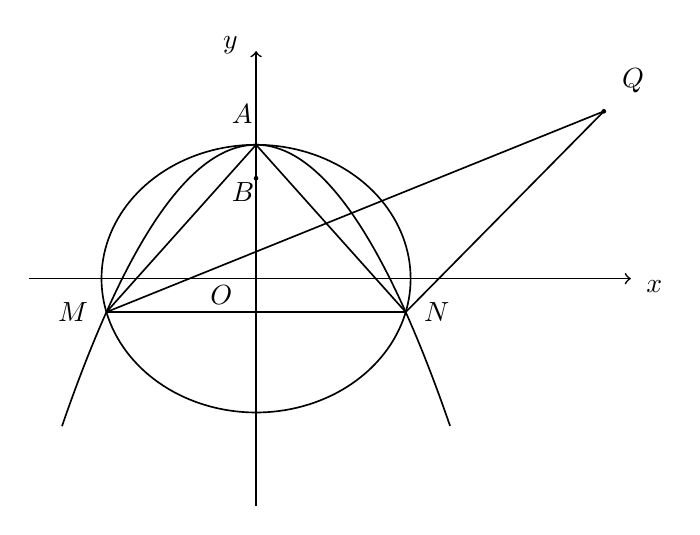
\begin{tikzpicture}[x=0.85cm,y=0.85cm,line width=.6pt]
\draw[->] (-3.4,0) -- (5.6,0) node[below=3pt,right=2pt] {$x$};
\draw[->] (0,-3.4) -- (0,3.4) node[above=2pt,left=3pt] {$y$};
\node[below left=4pt,xshift=-1pt,yshift=5pt] at (0,0) {$O$};
% ellipse C1: x^2/(16/3)+y^2/4=1, a=2.309,b=2
\draw[domain=0:360,samples=160,variable=\t] plot ({2.30940108*cos(\t)},{2*sin(\t)});
% parabola C2: x^2+2y=4 -> y=2-x^2/2
\draw[domain=-2.9:2.9,samples=140] plot (\x,{2-\x*\x/2});
\coordinate (M) at (-2.23606798,-0.5);
\coordinate (N) at (2.23606798,-0.5);
\coordinate (A) at (0,2);
\coordinate (B) at (0,1.5);
\coordinate (Q) at (5.19615242,2.5);
\fill (B) circle (0.035);
\fill (Q) circle (0.035);
\draw (M) -- (N);
\draw (M) -- (Q);
\draw (N) -- (Q);
\draw (A) -- (M);
\draw (A) -- (N);
\node[left=3pt] at (M) {$M$};
\node[right=3pt] at (N) {$N$};
\node[above=3pt,xshift=-5pt,yshift=1pt] at (A) {$A$};
\node[left=2pt,xshift=5pt,yshift=-5pt] at (B) {$B$};
\node[above right=3pt] at (Q) {$Q$};
\end{tikzpicture}
